
% NOTE - writing this in third person, as it is a report

% Chapter 3  Design

% Introduction – overview of the system 
% System architecture – include a diagram and discuss the main components in turn. (choice of approaches here)
% Discussion of design decisions
% Discussion of the data being used

\begin{comment}
    
- Technologies and Languages used

- System Architecture
    - System Architecture Diagram
    - System Architecture Components

- Recommmendation System
    - Content-based Filtering
    - Collaborative Filtering


- Data & Data Processing

- User Interface
    - Gradio
    - User Interface Design
    - User Interface Components




Python was chosen for this project due to its powerful capabilities in data manipulation and processing.
Additionally, I personally had a strong desire to work with Python, as it was an excellent opportunity to enhance my proficiency in the language.


\end{comment}
\section{System Architecture}
The system architecture is designed to be modular, allowing for the addition of other systems or components.
\label{sec:system_architecture}
\begin{figure}[H]
    \centering
    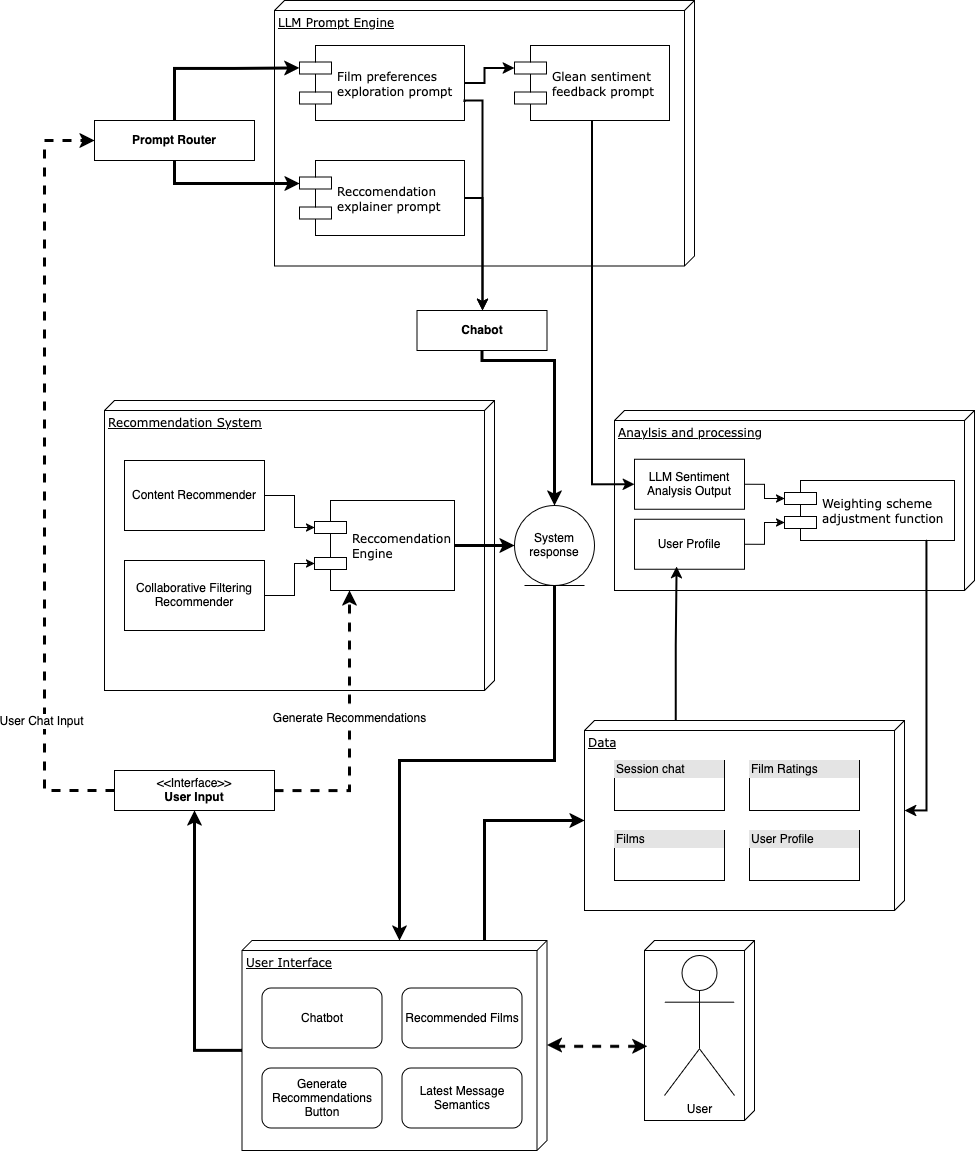
\includegraphics[width=0.9\textwidth]{Figures/FYP_HLA-Final.png}
    \caption{System Architecture Diagram}
    \label{fig:system_architecture_diagram}
\end{figure}
The system architecture diagram (\cref{fig:system_architecture_diagram}) shows the main components of the system, and how they interact with each other.


\subsection{System Architecture Components}
The system architecture is designed to be modular, allowing for the addition of new features and the adjustment of existing features.

\begin{itemize}
    \item \textbf{User Interface} - The user interface is designed to be simple and easy to use, allowing the user to interact with the system and provide feedback.
    \item \textbf{Recommendation System} - The recommendation system is designed to be modular, allowing for the addition of new recommendation systems, features and the adjustment of existing features.
    \item \textbf{Data} - The data holds the session conversation logs, user preference profile, films and their features, and film ratings from users.
    \item \textbf{Data Analysis \& Processing} - The data analysis and processing handles loading the data, processing sentiment analysis and adjustment of the user profile.
    \item \textbf{Large Language Model Prompt Engine} - The large language model prompt engine handles various scenarios, and routes the conversation to the appropriate component.
\end{itemize}

\section{Hybrid Recommendation System}
\label{sec:recommendation_system_design}
The recommendation system is designed to be both modular and adjustable. 
As there doesn't exist an existing framework, the recommendation system is designed to be a proof of concept, and is not intended to be the best implementation.
It provides a working implementation of a recommendation system, on which the other components can be built.
\\\\
The recommendation system is designed to have a hybrid recommendation system, using both collaborative filtering and content-based filtering.
This is to provide a more comprehensive recommendation system, allowing for the use of both collaborative filtering and content-based filtering features.

\subsection{Content-based Filtering}
\label{sec:content_based_filtering_design}
As there's no frameworks or libraries for content-based filtering with the adjustability needed for recommendation, explanation and feature adjustment, a custom implementation was needed.

As mentioned in \cref{sec:recommendation_system_design}, this implementation is just to act as a implementation that provides recommendations based on the features of the films.
The content-based filtering system uses the following features:
\begin{itemize}
    \item Genres
    \item Directors
    \item Cast
\end{itemize}
Additional features could be added, such as the release year, but the listed features are sufficient for a substantial proof of concept.
Adding additional features would be a stretch goal, and would not be necessary for the proof of concept.
\\\\
The content-based filtering system will fulfill the following requirements:
\begin{itemize}
    \item The system is able to provide recommendations based on the features
    \item The system can provide recommendations based on the features with a user profile
    \item Feature weights can be adjusted to provide different recommendations
    \item The system provides a breakdown of the scores for each feature in the recommendation
\end{itemize}
With this in mind, the content-based filtering system will not be forensically examined, the evaluation of the system will be covered in \cref{sec:recommendation_system_evaluation}.


\subsection{Collaborative Filtering}
\label{sec:collaborative_filtering_design}
For the collaborative filtering component of the recommendation system, the project uses the LensKit library\cite{ekstrand_2020_lenskit} for the collaborative filtering recommendation system.
It is a user-user collaborative filtering system, which uses the user-item matrix to find similar users and recommend items based on their preferences.

Again, as the recommendation system is only there to provide a working implementation of a recommendation system with key features, the collaborative filtering system is not the main focus of the project.
As such, the design is not intended to be the most efficient or effective implementation, but rather a 
it is not intended to be necessarily the best recommendation system, there is little need to evaluate the recommendation system in detail.

\section{Data}
\label{sec:data_design}
For the data, the project will utilise user ratings, film features, and user profiles.


\subsection{Data Storage}
\label{sec:data_storage_design}

Session vs User Profile data persistence
A user profile can have diffrent sessions, to suit their preferences depending on the context of the of the conversation or situation.
For example, a user may have a session for their kids, a session for their personal preferences, and a session for watching with their partner.
This allows for the user to have different preferences for different situations, and allows for the user to have a more personalized experience.


\section{User Interface}
\label{sec:user_interface_design}
The user interface is designed to be simple and easy to use, allowing the user to interact with the system and provide feedback.

For this reason, the project will use Gradio \cite{abid2019gradio} as the user interface for the system.
Gradio is a Python library that allows for the creation of simple and easy to use user interfaces for machine learning models.
It is highly customizable, and allows for the creation of user interfaces that are easy to use and understand.

The user interface will feature components to allow the user to converse with the agent, request recommendations, and view both the recommendations and the extracted preferences from the conversation.

\subsection{User Interface Wireframe}
\label{sec:user_interface_wireframe}

\begin{figure}[H]
    \centering
    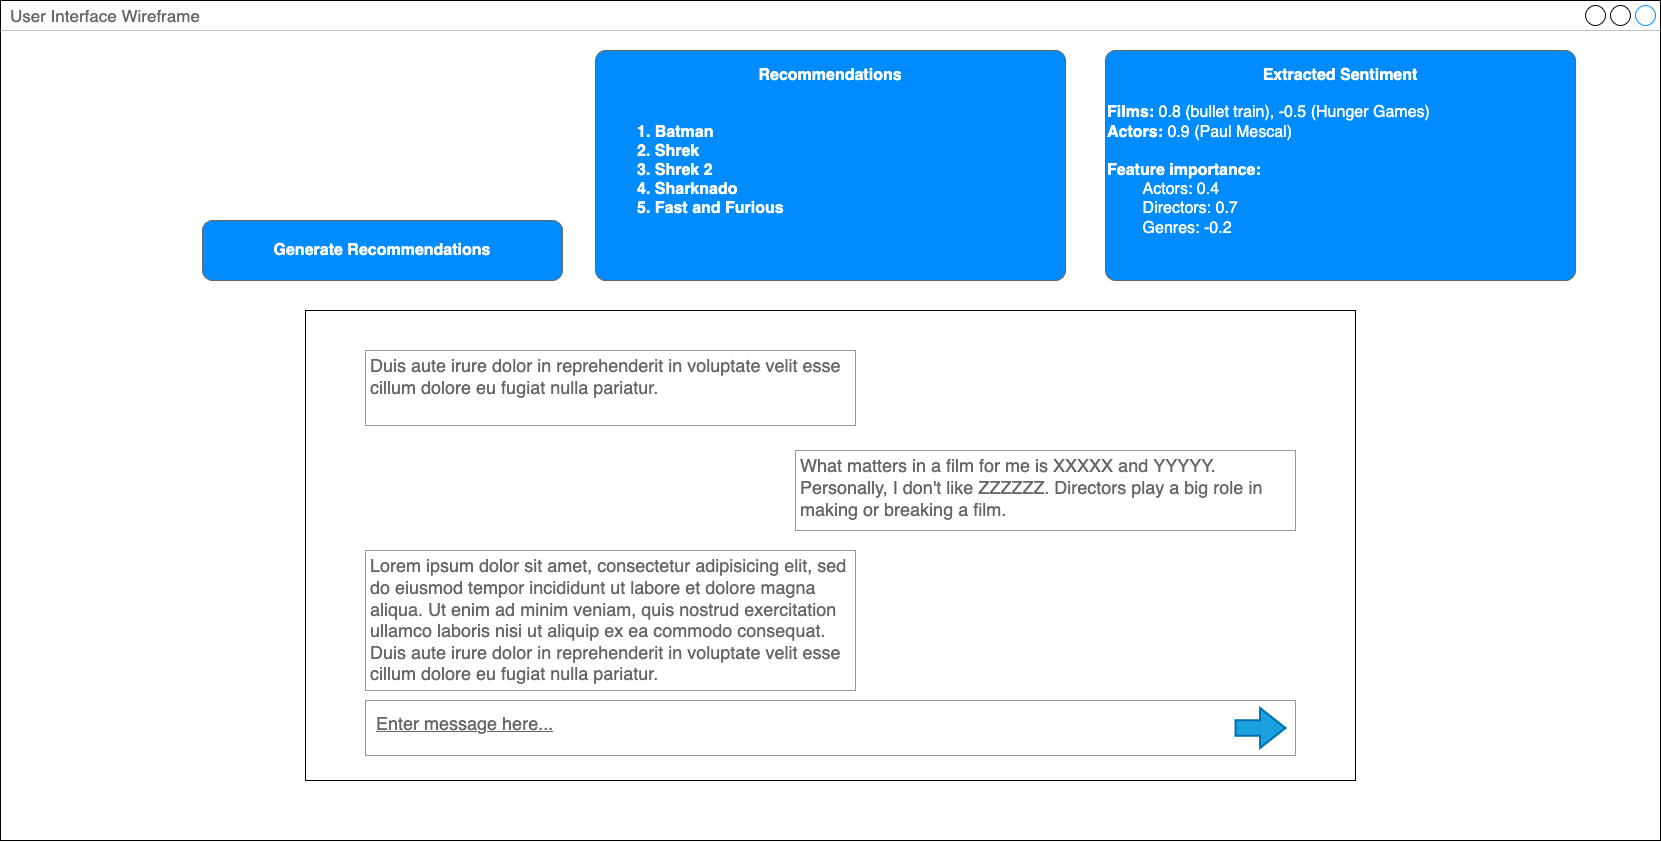
\includegraphics[width=1\textwidth]{Figures/UserInterface.png}
    \caption{Intended User Interface Wireframe}
    \label{fig:user_interface_design}
\end{figure}
